% !TEX root = ../main/main.tex
\section{Results and discussion}
 
 \begin{figure}[h]
 \begin{subfigure}[t] {0.23\textwidth}
 \centering
 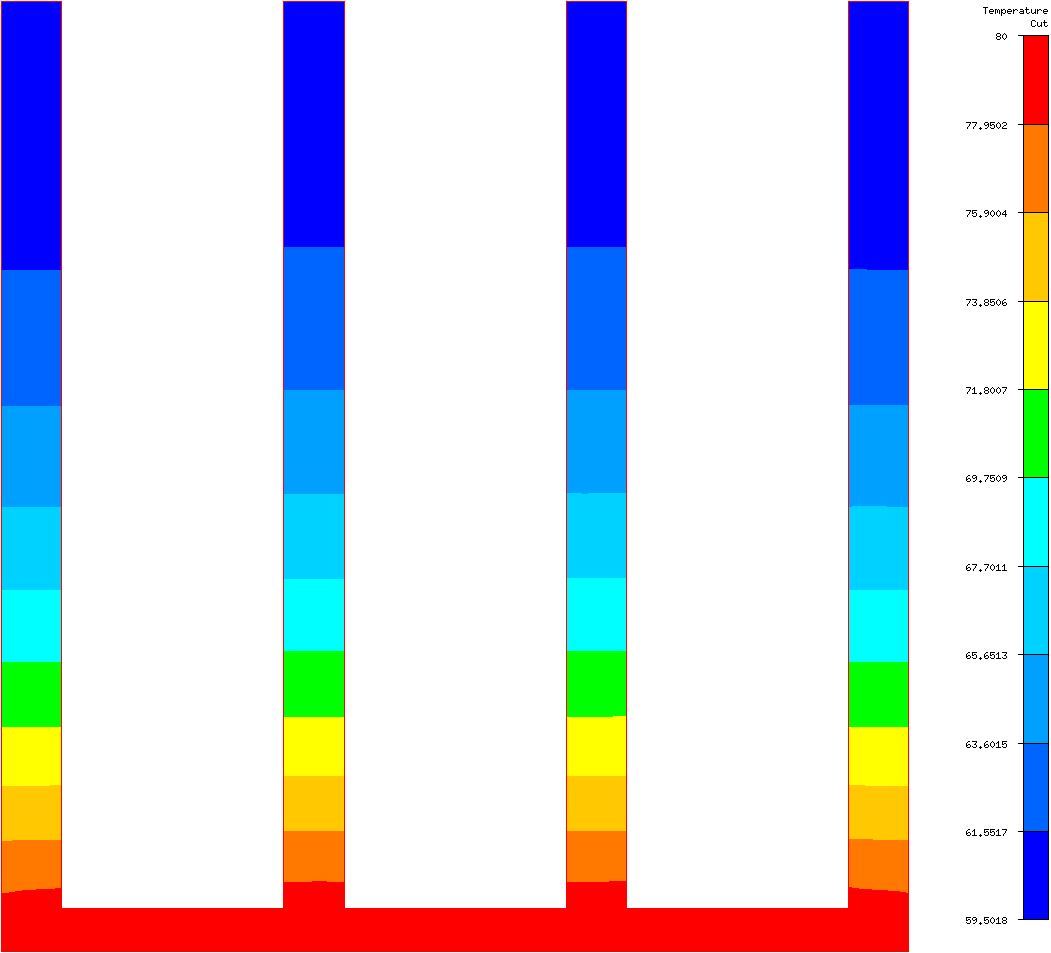
\includegraphics[width=0.7\textwidth]{../figures/heatsink4_h105_gmf005.png}
 \caption{4 fins, 1 height}
 \label{fig:mesh_temps_res_4_1}
 \end{subfigure}
 ~
  \begin{subfigure}[t] {0.23\textwidth}
 \centering
 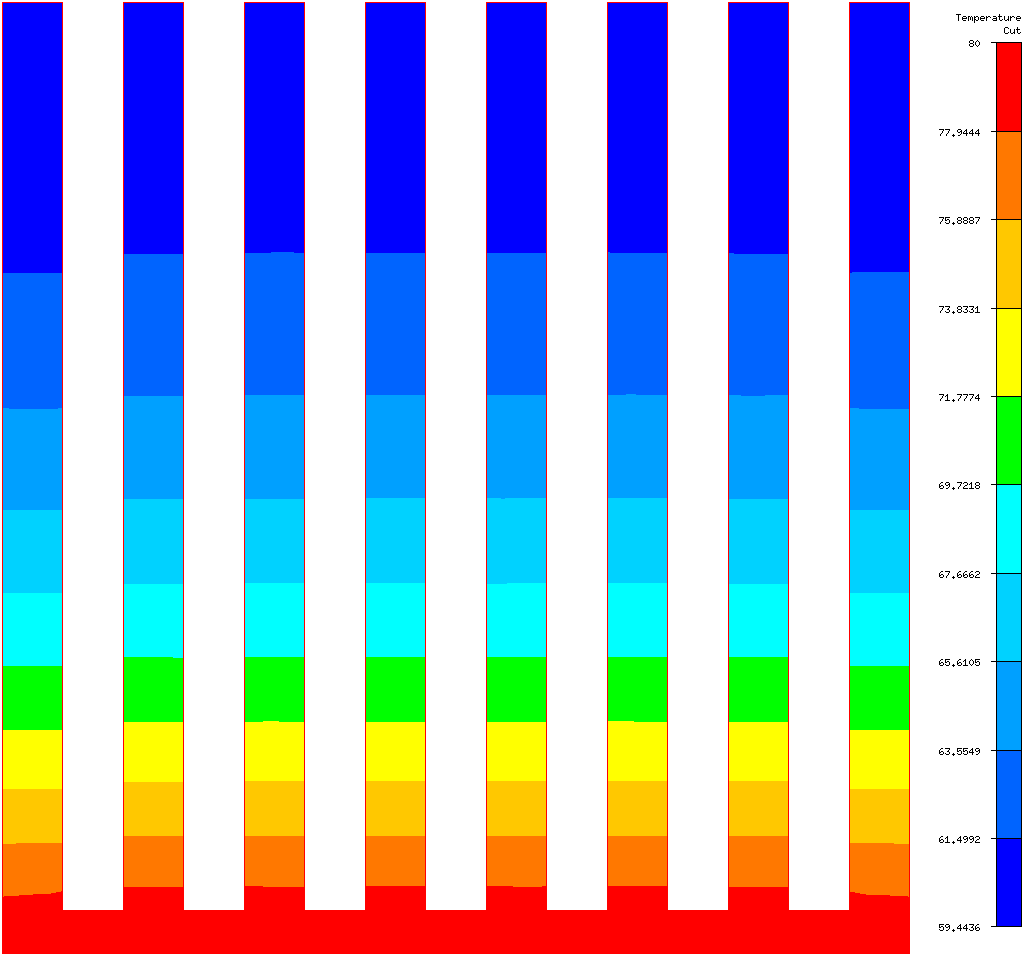
\includegraphics[width=0.7\textwidth]{../figures/heatsink8_h105_gmf005.png}
 \caption{8 fins, 1 height}
 \label{fig:mesh_temps_res_8_1}
 \end{subfigure}
 ~
 \begin{subfigure}[t] {0.23\textwidth}
 \centering
 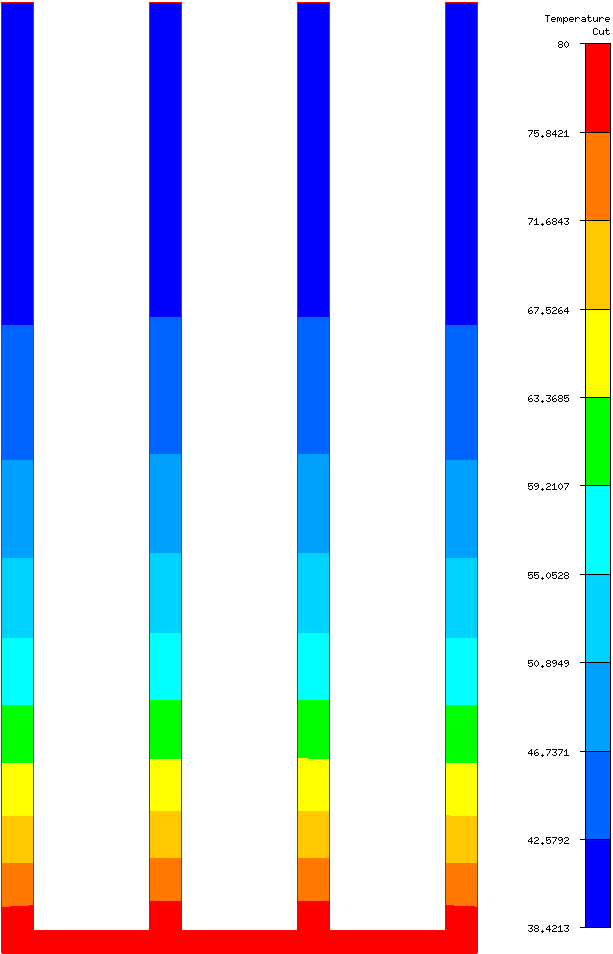
\includegraphics[width=0.7\textwidth]{../figures/heatsink4_h205_gmf005.png}
 \caption{4 fins, 2 height}
 \label{fig:mesh_temps_res_4_2}
 \end{subfigure}
 ~
 \begin{subfigure}[t] {0.23\textwidth}
 \centering
 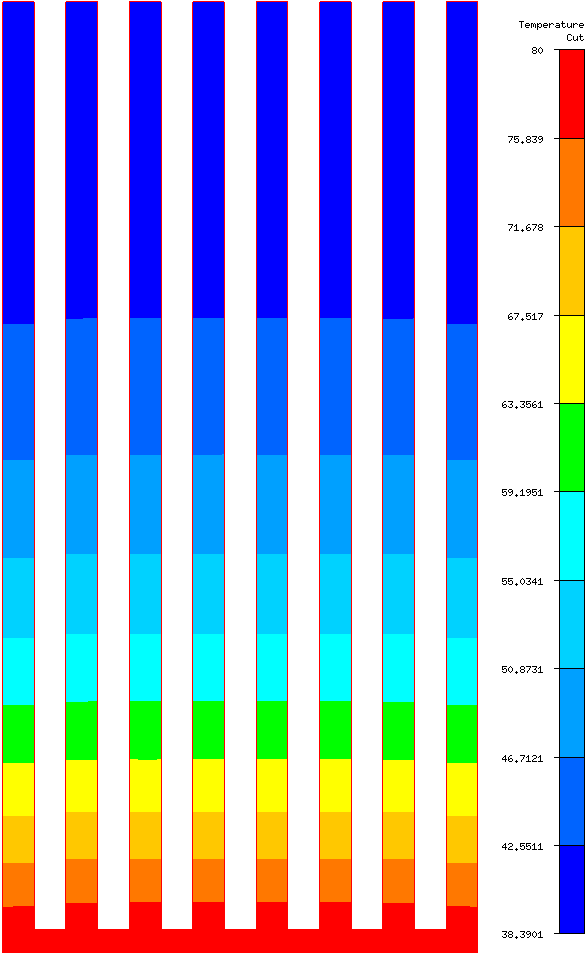
\includegraphics[width=0.7\textwidth]{../figures/heatsink8_h205_gmf005.png}
 \caption{8 fins, 2 height}
 \label{fig:mesh_temps_res_8_2}
 \end{subfigure}
 \caption{Temperatures in the middle of the heat sink for the different meshes.}
 \label{fig:mesh_temps}
 \end{figure}
 
\subsection{Visualization of results}
Visualizing results from simulations is important in order to understand the result. when having a function in three dimensions it is necessary to make choices of what part of the result which should be displayed. The natural way of doing this is either with iso-surfaces or cutting-planes. The geometries in \ref{fig:meshes} are somewhat symmetric, especially along the fins, which suggests that the temperature field should be more or less constant along this axis. In 3D visualizing software this is easier to see, and in our solution this is indeed the case. Therefore figure \ref{fig:mesh_temps} represents a cutting plane normal to the find, which should give a good representation of the temperature field in the whole geometry.

\subsection{Assumptions and Physical Interpretation}
In our analysis we have made some assumptions and initial choices for the boundary conditions to make a somewhat simplified mathematical model. For the temperature of the bottom of the heat sink base we enforced a constant Dirichlet boundary condition of \SI{80}{\celsius}. This choice was made because it is an estimate of the temperature of a very warm processor working at maximum capacity. By enforcing Dirichlet boundary condition we disallow the hypothetical processor to actually cool down, which is not necessarily a realistic assumption. When looking at a computer processor it would be natural to want to keep the temperature below some maximum threshold, and look at how the heat sink would need to be engineered in order to have a sufficient heat loss below this temperature. In that case some kind of Neumann boundary condition on the bottom would  maybe be better suited if you want to see such a cooling effect.

Another modeling choice made regarding the Robin conditions on the rest of the boundary is that the ambient temperature in the description of the boundary value problem \eqref{eq:heat_bvp} is also constant. This means that even in the tight spaces in between the fins the air temperature is constant. You could think of it as an average temperature on the boundary. One could maybe improve on this assumption by enforcing different ambient temperature on the outer boundary and the boundary in between the fins. Besides you would probably need a very powerful fan to transport the heat away to keep the ambient temperature at 20 degrees as assumed here.
If there were many more fins and they were a lot thinner and closer together it would be a good point to take into account the heat radiation from one fin to another. Also there would be challenges regarding the mesh. Using tetrahedron elements one could expect the elements to become very irregular. A solution could be to use brick prism elements, or alternatively a 2D mesh of the flat fins.

In figure \ref{fig:mesh_temps} we can see the temperatures for the different meshes. The temperature ranges from about \SI{59}{\celsius} to \SI{80}{\celsius} for figure \ref{fig:mesh_temps_res_4_1} and \ref{fig:mesh_temps_res_8_1}, and from \SI{39}{\celsius} to \SI{80}{\celsius} for figure \ref{fig:mesh_temps_res_4_2} and \ref{fig:mesh_temps_res_8_2}. The Dirichlet boundary on the bottom works like a thermal reservoir, supplying as much heat as possible, so the temperature profiles along the fins are virtually identical between fins of the same height, regardless of the number of fins.

The total heat loss to the surrounding air is
\begin{equation}
    \int_{\partial\Omega_R}\! \pdv{u}{n}\, \mathrm{d}{\gamma}.
\end{equation}
Since the heat flux in Robin boundary condition in equation \eqref{eq:heat_bvp} is proportional to the temperature difference, and we want the to maximize the heat loss, a high temperature is preferred. The heat sink in figure \ref{fig:mesh_8_1} and \ref{fig:mesh_4_2} have both the same surface area and the same volume,  however from figure \ref{fig:mesh_temps_res_8_1} we see that \ref{fig:mesh_8_1} generally have a higher temperature. The result is that \ref{fig:mesh_8_1} in total has a greater heat loss. It would appear that, given a certain amount of material, the heat sink should be designed with many short, thin fins, as opposed to a fewer and higher fins.